\label{ordernsquared}
Elementary sorts are also referred to as $O(N^2)$ sorts. This is due to the
manner in which they check every key in the array in order to sort a single key;
for every key to be sorted, every other key is checked.  Four of these sorts are
discussed here. They are insertion sort, selection sort, bubblesort and
shakersort.

\section{Selection sort}

Selection sort works in a straightforward manner. It begins by 
searching the unsorted array for the smallest key, then swapping it into the
first position in the array. This key is now the first element of a sorted
array, being built from the left. The remainder of the array is
still unsorted, and it is now searched for its smallest key, which is swapped
into place. This continues until the entire array is sorted. Sample code is in
Figure \vref{Selection sort code}.

\code{Selection sort code}{on2_selectsort.c}
\subsection{Testing}
All elementary sorts are only sorted up to 65536 keys in the simulations, and
262144 keys with the performance counters. Due to the quadratic nature of
these sorts, days and weeks would be required to run tests on the larger arrays.

\subsubsection{Expected Performance}
Sedgewick provides a discussion on the performance of elementary sorts. The
observations on instruction count are his, and come from \cite{Sedgewick02}.

Selection sort uses approximately $N^2/2$ comparisons and exactly $N$ exchanges.
As a result, selection sort can be very useful for sorts involving very large
records, and small keys. In this case, the cost of swapping keys dominates the
cost of comparing them. Conversely, for large keys with small records, the cost
of selection sort is far higher than for other simple sorts.

The performance of selection sort is not affected by input, so the instruction
count varies very little.  Its cache behaviour is also not affected by input,
and selection sort performs very badly from a cache perspective. There are $N$
traversals of the array, leading to bad temporal reuse. If the array doesn't fit
inside the cache, then there will be no temporal reuse.

The level 1 cache should have bad performance as a result. Since it is smaller
than the array, the performance of the level 1 cache should simulate the
performance of the level 2 cache.

\label{selection branches logn}
The branch prediction performance is not expected to be bad. Flow control
predictions are very straightforward, and should result in very few misses.
Comparison predictions, however, are very numerous. Each array traversal has an
average of $N/2$ comparisons, and approximately $log_2(N/2)$ of them should be
taken, while the rest are not-taken. The taken predictions will be misses,
while the rest should be hits, so it is expected that there will be $logN$
misses per key.

This number is not immediately obvious. Consider a single step of the selection
sort. The first key to be sorted is, on average, larger than half the keys and
smaller than the other half, so it will have to travel across half the array to
find a key smaller than it, on average. Once it finds a smaller key, this will
be larger than a quarter of the keys in the array, and so it will need to travel
half of the remaining array, on average, before it finds it. The search will
continue like this until the entire array has been covered. Comparing two keys
and discovering that the new key is not smaller than the current smallest is the
norm; every time a smaller key is found a branch misprediction will occur (if
two or more keys in a row are successively smaller, this may not be the case).
The length of the array to be considered in $N/2$ on average, and an average
total of $Nlog_2(N/2)$ branch misses will occur. This assumes randomly sorted
keys.

%TODO look at knuths number here
TODO Knuth has a formula which I will look up.

\section{Insertion sort}

Insertion sort, as its name suggests, is used to insert a single key into its
correct position in a sorted list. Beginning with a sorted array of length one,
the key to the right of the sorted array is swapped down the array a key at a
time, until it is in its correct position. The entire array is sorted in this
manner.

An important improvement to insertion sort is the removal of a bounds check. In
the case that the key being sorted into the array is smaller than the smallest
key in the array, then it will be swapped off the end of the array, and continue
into the void. To prevent this, a bounds check must be put in place, which will
be checked every comparison, doubling the number of branches and severely
increasing the number of instructions. However this can be avoided by using a
sentinel. This is done by finding the smallest key at the start, and putting it
into place. Then no other key can be smaller, and it will not be possible to
exceed the bounds of the array. Another technique would be to put $0$ as the
smallest key, storing the key currently in that position, then putting it in
place at the end. This would use a different insertion sort, with a bounds
check, going in the opposite direction. The first of these is shown in the
sample code in Figure \vref{Insertion sort code}.

\code{Insertion sort code}{on2_insertsort.c}
\subsection{Testing}
\subsubsection{Expected Performance}
These instruction count observations are again due to Sedgewick.  Insertion sort
performs in linear time on a sorted list, or slightly unsorted list. With a
random list, there are, on average, there are $N^2/4$ comparisons and $N^2/4$
half-exchanges\footnote{A half-exchange is where only one part of the swap is
completed, with the other value stored in a temporary to be put in place later.}.
As a result, the instruction count should be high, though it is expected to be
lower than selection sort.

The cache performance should be similar to selection sort as well. While
selection sort slowly decreases the size of the array to be considered,
insertion sort gradually increases the size. However, each key is not checked
with every iteration. Instead, on average, only half of the array will be
checked, and there will be high temporal and spatial reuse due to the order in
which the keys are accessed. This should result in lower cache misses than
selection sort.

The flow control of insertion sort is determined by an outer loop, which should
be predictable, and an inner loop, which, unlike selection sort, is dependent on
data. As a result, the predictability of the flow control is highly dependant on
the predictability of the comparisons.

\section{Bubblesort}
Bubblesort, as its name suggests, works by bubbling small keys from right of
the array to the left. It begins by taking a key from the end and moving it left
while it is less than any keys it passes. Once it comes across a smaller key, it
changes to this key, and moves it towards the left of the array. In this way, every
iteration the smallest key moves left to its final position, and other small
keys are slowly moved left, so that the unsorted part of the array becomes more
sorted as bubble sort continues.

An improvement made to bubblesort is that it stops as soon as the array is
sorted. Sample bubblesort code is in Figure \vref{Bubblesort code}.

\code{Bubblesort code}{on2_bubblesort.c}
\subsection{Testing}
\subsubsection{Expected Performance}
These instruction count observations are again due to Sedgewick.  Bubblesort has
$N^2/2$ comparisons and exchanges. The number of passes over the array, and size
of each pass is the same as selection sort, and similar instruction count
results are expected.  The extra check to see if the array is sorted adds
$O(NlogN)$ instructions, but this is small in comparison to the number of
instructions saved if the sort ended early.

The cache performance of bubblesort should be the same as that of selection
sort. Each key loaded into the cache is used just once, and will be ejected from
the cache if the data set is large enough.

The branch predictive performance is also expected to be similar. While
selection sort has $O(NlogN)$ misses, each of bubblesort's comparisons has
the potential to be a miss, and not just in the pathological case. However, as
the sort continues and the array becomes more sorted, the number of misses
should decrease. The number of flow control misses should be very low.

\section{Bubblesort2}
Bubblesort2 incorporates an improvement to end bubblesort early. The bubblesort
implementation described in the previous section ends early if it detects that
the array is fully sorted.  It keeps a binary flag to indicate if there were any
exchanges along the way.  Instead, bubblesort2 keeps track of the last exchange
made, and starts the next iteration from there. This means that any pockets of
sorted keys are skipped over, not just if they occur at the end. Bubblesort2
code is shown in Figure \vref{Bubblesort2 code}.

\code{Bubblesort2 code}{on2_bubblesort2.c}
\subsection{Testing}
\subsubsection{Expected Performance}
It is expected that the bubblesort2 should perform faster than the original in
all metrics. Instruction count, were there no conditions that allowed keys to be
skipped, would be the same, as no extra instructions are added. The flow of the
algorithm is the same, though there should be fewer iterations, especially at
the start, when iterations are longer, so cache accesses, and branch misses
should be reduced along with instruction count.

\section{Shakersort}
Shakersort is sometimes called back-bubblesort. It behaves like a bubblesort
which moves in both directions rather than just one way. Both ends of the array
become sorted in this manner, with the larger keys slowly moving right and the
smaller keys moving left. Sample code for shakersort is shown in Figure
\vref{Shakersort code}.

\code{Shakersort code}{on2_shakersort.c}
\subsection{Testing}
\subsubsection{Expected Performance}
The instruction count of shakersort is expected to be exactly the same as
bubblesort. The version of shakersort used here, however, does not incorporate
the improvement to end the sort early if the array is already sorted. This will
probably slightly reduce the instruction count as the sort is unlikely to end
early for random keys. 

The cache performance of shakersort is expected to be superior to that of
bubblesort. A small amount of temporal reuse occurs at the ends of the array,
as each key is used twice once its loaded into the cache. In addition, when the
array is not more than twice the size of the cache, then the keys in the centre
of the array are not ejected from the cache at all.

Finally, the branch prediction results are expected to be the same as in bubble
sort, with one difference.  Keys which must travel the entire way across the
array are taken care of earlier in the sort. If the largest key is in the
leftmost position, it must be moved the entire way right, which causes misses
for every move in bubblesort, since each move is disjoint from the next. In
shakersort, however, each in the correct direction will follow a move in the
same direction, each of which should be predicted. This works for a lot of
keys, which are more likely to move in continuous movements than they are in
bubblesort, where only small keys on the right move continuously. The
performance should improve noticeably as a result.

\section{Shakersort2}
Shakersorts incorporates the same improvements over shakersort as bubblesort2
does over bubblesort, that is, it skips over pockets of sorted keys in both
directions, as well as ending early. The code for shakersort2 is in Figure
\vref{Shakersort2 code}.

\code{Shakersort2 code}{on2_shakersort2.c}
\subsection{Testing}
\subsubsection{Expected Performance}
It is expected that the improvements will make shakersort faster in all cases
than its original form.

\section{Simulation Results}

%TODO check that this is put in after the titlepage
%TODO check that the captions are the same as the captions at the end of the
%other chapters
% I'm doing a slightly different result here. Level 2 doesn't interest us, so put
% in 2 prediction results instead - 1 for select/insert, 1 for bubble/shaker
\afterpage{
\label{Elementary sort results}

\thispagestyle{empty}
\clearpage
\enlargethispage{14em}
\vspace*{-8em}
\begin{figure}[H]
\begin{changemargin}
\subfigure[Cycles per key - this was measured on a Pentium 4 using hardware performance counters.]
{\label{elementary cycles}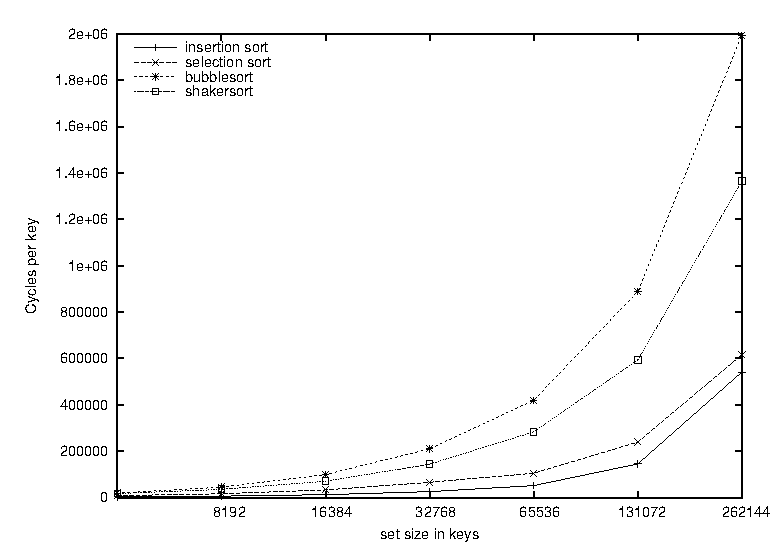
\includegraphics[scale=\myscale]{plots/on2_-_cycles.eps}}
\subfigure[Instructions per key - this was simulated using SimpleScalar \cc{sim-cache}.]	
{\label{elementary instructions}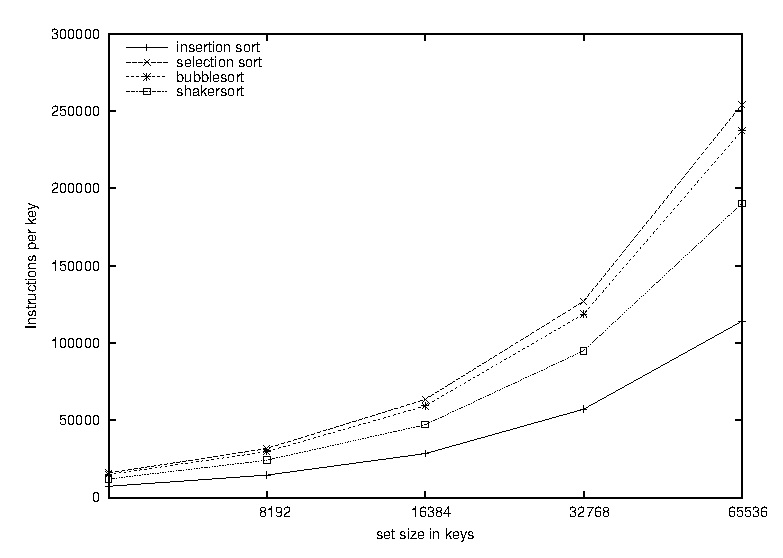
\includegraphics[scale=\myscale]{plots/on2_-_Instructions.eps}}
\end{changemargin}
\vspace*{6em}
\caption{Simulated Instruction count and empiric cycle count for elementary sorts}
\label{Simulated Instruction count and empiric cycle count for elementary sorts}
\end{figure}
\newpage

\thispagestyle{empty}
\clearpage
\enlargethispage{14em}
\vspace*{-8em}
\begin{figure}[H]
\begin{changemargin}
\subfigure[Level 1 cache misses per key - this was simulated using SimpleScalar \cc{sim-cache}, simulating an 8KB data
cache with a 32 byte cache line and separate instruction cache.]
{\label{elementary level 1 misses}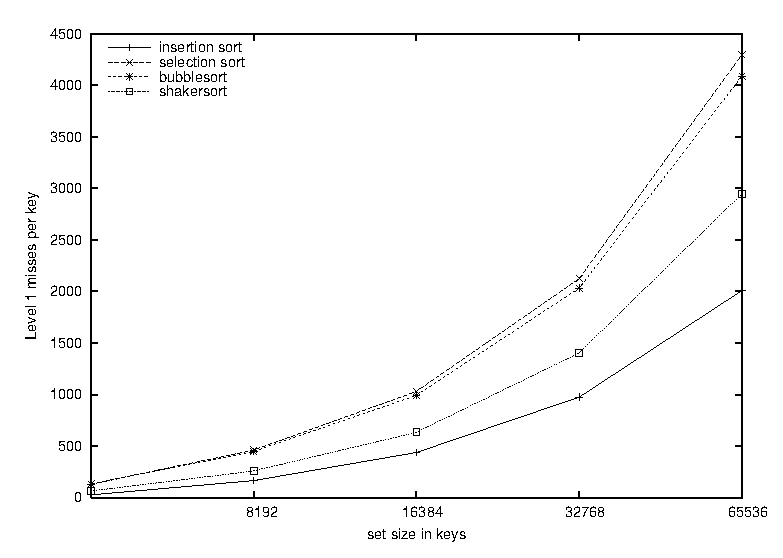
\includegraphics[scale=\myscale]{plots/on2_-_Level_1_misses.eps}}
\subfigure[Branches per key - this was simulated using \cc{sim-bpred}.]
{\label{elementary branches}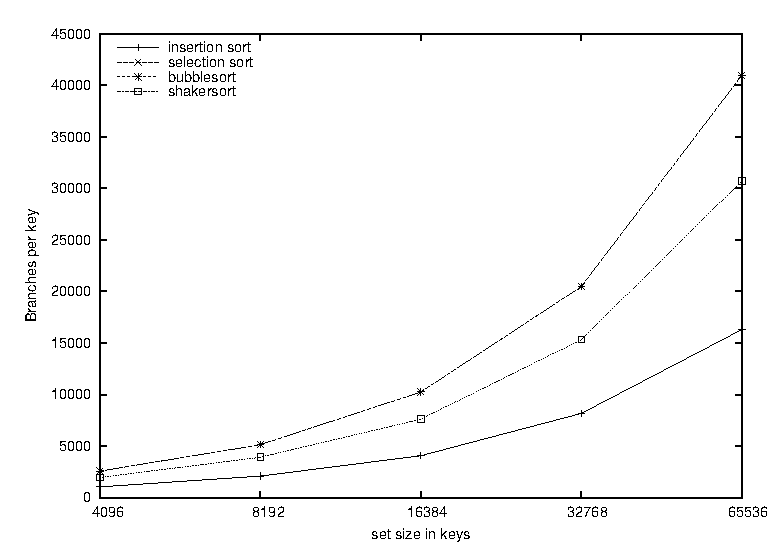
\includegraphics[scale=\myscale]{plots/on2_-_Branches.eps}}
\end{changemargin}
\vspace*{6em}
\caption{Cache and Branch prediction simulation results for elementary sorts}
\label{Cache and Branch prediction simulation results for elementary sorts}
\end{figure}
\newpage

\thispagestyle{empty}
\clearpage
\enlargethispage{14em}
\vspace*{-8em}
\begin{figure}[H]
\begin{changemargin}
\centering
\subfigure[Branches misses per key - this was simulated using \cc{sim-bpred}, with bimodal and two-level adaptive
predictors. The simulated two-level adaptive predictor used a 10 bit branch history register which was XOR-ed with the
program counter.]
{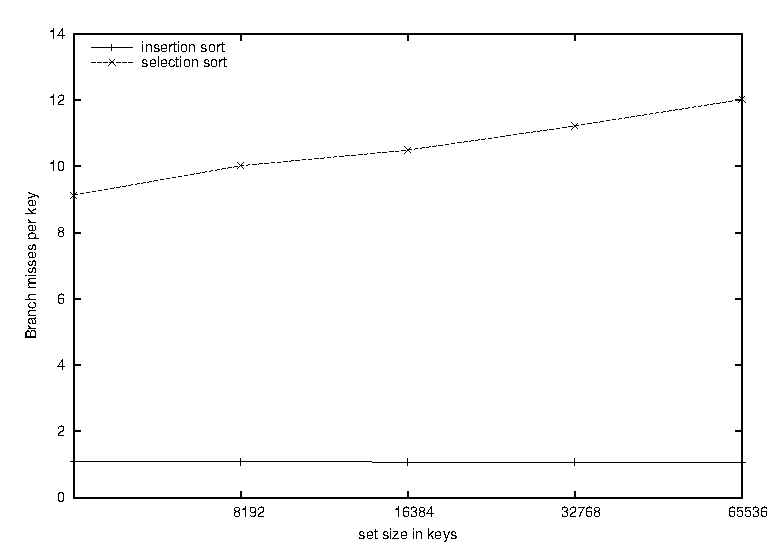
\includegraphics[scale=\myscale]{plots/on2_-_Branch_misses1.eps}}
\subfigure[Branches misses per key - this was simulated using \cc{sim-bpred}, with bimodal and two-level adaptive
predictors. The simulated two-level adaptive predictor used a 10 bit branch history register which was XOR-ed with the
program counter.]
{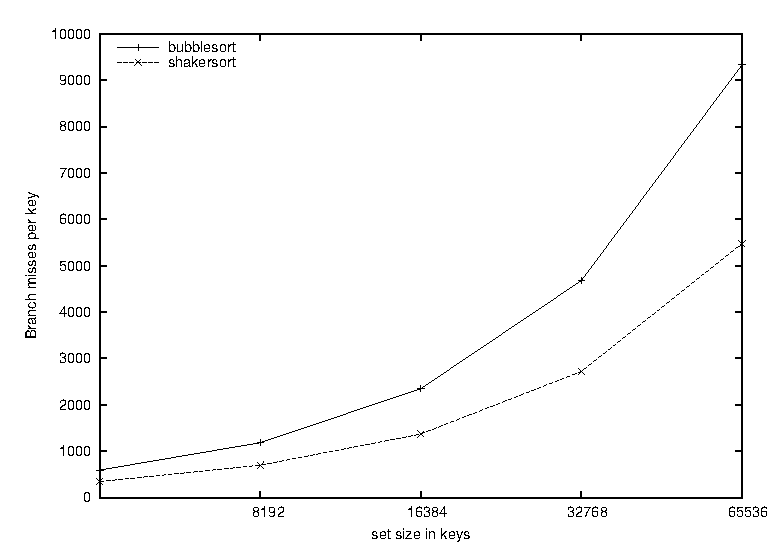
\includegraphics[scale=\myscale]{plots/on2_-_Branch_misses2.eps}}
\end{changemargin}
\vspace*{6em}
\caption{Branch Simulation results for elementary sorts}
\label{Branch Simulation results for elementary sorts}
\end{figure}
}

Figure \ref{elementary instructions} shows the instruction count of each
elementary sort. Each sort's instruction count is as predicted. Selection sort
has the most instructions, and insertion sort has approximately half that
number, as predicted. Bubblesort has almost the same number of instructions as
selection sort, but shakersort has a significant number less. The improvement to
bubblesort in bubblesort2 have increased the instruction count, contrary to
predictions, and similarly in the shakersort2.

The level 2 cache performance of these sorts is not considered, as the set sizes
are never larger than the level 2 cache. Instead, the level 1 caches are used,
and their performance can be used to approximate the level 2 cache in these
cases. These results are shown in Figure \ref{elementary level 1 misses}. Each
set size is larger than the cache, and each sort iterates across the entire
array each time, leading to very poor performance.

As expected, selection sort is the worst. This is due to the fact that it
considers the entire unsorted segment of the array for each key to be put in
place. Bubblesort, with similar behaviour, is only slightly better. Shakersort
has a small amount of temporal reuse (see Section \ref{temporal locality}),
reducing its number of misses. Shakersort2 is placed roughly between insertion
sort and shakersort, showing that ending early is helpful in its case. This does
not appear to be the case with bubblesort2 though, which performs identically to
bubblesort.

Insertion sort performs best of these sorts in relation to cache misses. This
is due to the fact that the keys it considered most recently are used again for
the next key. These keys will be swapped out fairly regularly, however, but not
nearly as often as selection sort, where they are swapped out at nearly every
iteration.

Figure \ref{elementary branches} shows the number of branches per key of these
sorts, while Figure \ref{Branch Simulation results for elementary sorts} shows
the branch misses per key.  Branch prediction performance is not surprising.
Each sort has a similar number of branches, with insertion sort having half as
many as selection and bubblesort, and shakersort being half-way between the
two. The number of misses for bubblesort and shakersort are huge; nearly one in
four comparisons are misses. As the data sets gets large, there are nearly
10,000 branch misses involved in sorting a single key. The improved bubblesort
had exactly the same number of misses and branches. The improved shakersort has
a lot less branches, but the same number of misses. This is because skipping
over sorted keys is predictable from the first branch miss.

Selection sort, meanwhile, has the same number of branches as bubblesort, but
only $O(logN)$ misses per key. The most interesting result, though, is insertion
sort. This has exactly one miss per key. Although this result was not predicted
in advance, on reflection this behaviour is obvious: every iteration involves
moving the key left. The only time it will not move left is when its being put
into place, and this only happens once for every key. This shows that it is
possible to completely eliminate even comparative branch misses. It also
establishes insertion sort as the best of the simple sorts, and it is used later
in quicksort and mergesort as a result of this. \label{insertion is
predictable}

Another interesting result comes from a comparison between shakersort and
selection sort. The number of cycles to sort an array (shown in Figure
\ref{elementary cycles}) is nearly twice as high on shakersort as it is for
selection sort. Shakersort has a significantly lower instruction count and cache
miss count than selection sort, but has several orders of magnitude worse branch
misses. This shows how important it is to consider branch misses in an
algorithm, especially comparative ones. It also establishes that exchange-based
algorithms, such as bubblesort and shakersort, will perform considerably worse
than algorithms which have a correlation between successive branches, as in
insertion and selection sorts.

\section{Future Work}
Simulations from elementary sorts take a lot of time. Running the simulation for
bubblesort with 65536 keys takes nearly a day, and the simulation for 4194304
keys would take nearly 11 years to run. Due to this, it is necessary to
extrapolate results for larger data sets from the results from these smaller
sets. The only place where it's necessary to have larger data sets is in the
case of cache results. The cache behaviour of these sorts should change
dramatically once the keys no longer fit in the cache, as they do in subsequent
chapters with other sorts. The results can be simulated, by using a
smaller cache, but in this case all the data sets are too large. It would be
easy to use data sets smaller than the cache, but in this case many factors
would not have time to be amortised, such as filling the cache and branch
prediction tables.

Each of these sorts could have the number of iterations across the array reduced
by a half or a third by considering two or three keys at a time. The resultant
reduction in cache misses is predictable, and instruction count should reduce.
The new branch prediction results, especially in the case of insertion sort, may
be significantly worse, or may stay the same. The results of this would be
interesting.

It should be possible to make more cache-conscious versions of these sorts.
Making a bubblesort which performs a bubble across an entire cache line would
be an example. However, these would only make a difference on large data sets,
when better sorts such as quicksort should be used. In addition, the complexity
of doing this means it may be easier to code a simple $O(NlogN)$ sort, which
would perform better for the same effort. Due to this, a cache-conscious
elementary sort is but an academic exercise.
